\documentclass[13pt]{beamer}				\usepackage{graphicx}
\usepackage{comment}
\usepackage{pdfpages}	
\usepackage{tikz}
\usepackage{comment}
\usepackage{relsize}
\usepackage{mathtools}
\usepackage{biblatex}
\addbibresource{biblio.bib}

\newcommand\Ccancel[2][black]{\renewcommand\CancelColor{\color{#1}}\xcancel{#2}}
\mode<presentation>						% Set options
{
  \usetheme{Madrid}					% Set theme
  \usecolortheme{seahorse} 				% Set colors
  \usefonttheme{default}  				% Set font theme
  \setbeamertemplate{caption}[numbered]	% Set caption to be numbered
}
\usepackage[makeroom]{cancel}
\definecolor{blue}{RGB}{88, 88, 191}
\definecolor{white}{RGB}{255, 255, 255}
\definecolor{uuuuuu}{rgb}{0.2666,0.2666,0.2666}
\definecolor{wwwwww}{rgb}{0.4,0.4,0.4}
\definecolor{ccqqqq}{rgb}{0.8,0,0}
\definecolor{qqqqff}{rgb}{0,0,1}


\usepackage{hyperref}					% For cross-referencing

\title[Learning the Pareto front with hypernetworks]{Learning the Pareto Front with Hypernetworks}
\author[Polina Barabanshchikova]{Polina Barabanshchikova}	
\institute[MIPT]{MIPT}
\DeclareMathOperator{\rank}{rank}
\DeclareMathOperator{\dist}{dist}
\DeclareMathOperator{\conv}{conv}
\DeclareMathOperator{\tr}{tr}
\DeclareMathOperator{\degree}{deg}
\DeclareMathOperator{\cl}{cl}
\DeclareMathOperator{\argmin}{argmin}
\DeclareMathOperator{\lo}{\longleftrightarrow}
\DeclareMathOperator{\Lo}{\Longleftrightarrow}
\newcommand{\D}{\overline{D}}
\begin{document}

\begin{frame}
  \titlepage
\end{frame}

\begin{frame}{Multi-objective Optimization (MOO)}
%\textbf{Multi-objective optimization (MOO)} aims to optimize several possibly conflicting objectives.
%\begin{block}{Multi-objective optimization}
%\end{block}
\begin{itemize}
\item MOO is defined by $m$ losses $\boldsymbol\ell = (\ell_1, \dots, \ell_m)$, $\ell_i : \mathbb{R}^d \rightarrow \mathbb{R}_+$%, $i = 1, \dots, m$
\item A partial ordering is defined on the loss space 
$$\boldsymbol\ell (\theta_1) \preceq \boldsymbol\ell (\theta_2) \text{ if } \ell_i(\theta_1) \leq \ell_i(\theta_2) \text{ for all } i$$ 
\item A point $\theta_1 \in \mathbb{R}^d$ dominates $\theta_2 \in \mathbb{R}^d$ if $\boldsymbol\ell (\theta_1) \prec \boldsymbol\ell (\theta_2)$, that is
$$\boldsymbol\ell (\theta_1) \preceq \boldsymbol\ell (\theta_2) \text{ and } \ell_i(\theta_1) < \ell_i(\theta_2) \text{ for some } i$$ 
%\item Pareto optimal point -- not dominated by any other point
%\item Pareto front -- set of all Pareto optimal solutions
\end{itemize}
\end{frame}

\begin{frame}{Pareto Optimality}
\begin{itemize}
\item \textit{Pareto optimal point} -- not dominated by any other point
\item \textit{Pareto front} -- set of all Pareto optimal solutions
\end{itemize}
\begin{figure}[h!]
    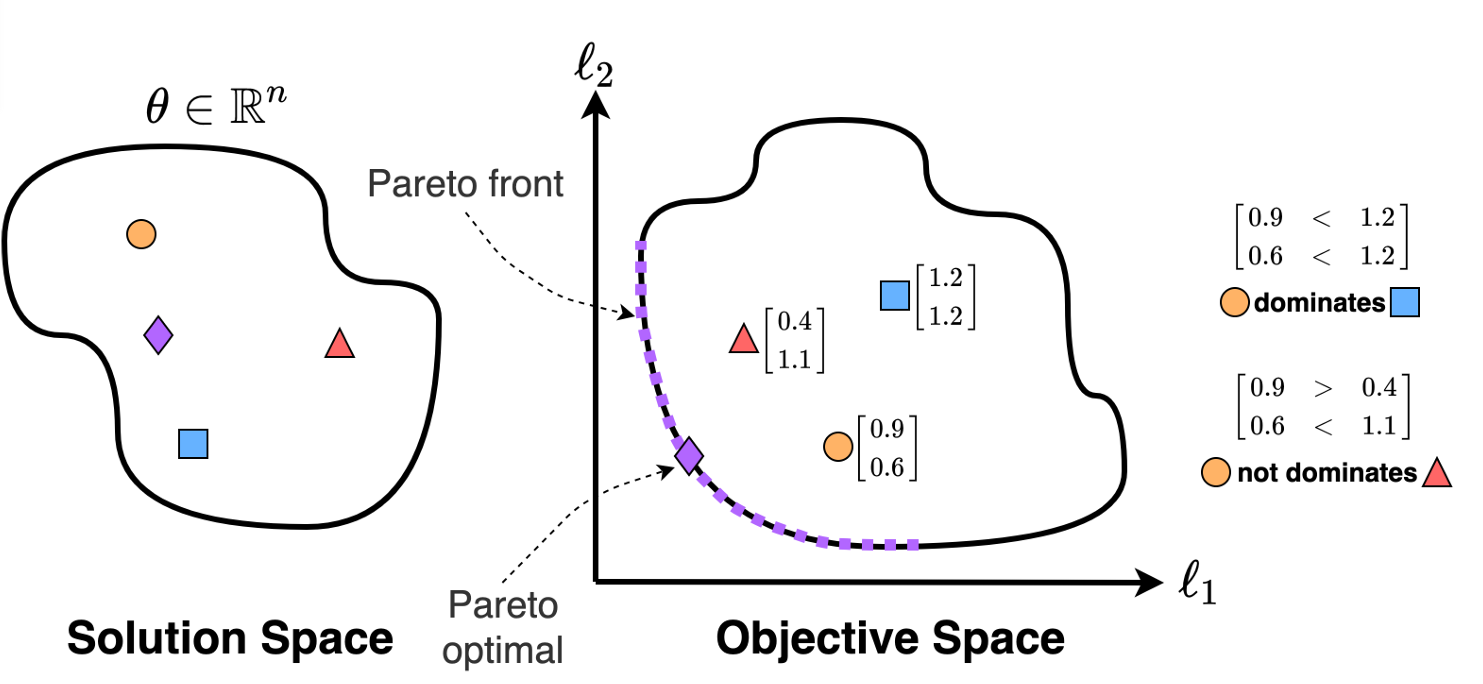
\includegraphics[width=0.7\textwidth, trim={0 0 0 0cm},clip]{images/pareto_front.png}
\end{figure}
\end{frame}

\begin{frame}{Exact Pareto Optimality}
\begin{itemize}
\item Each optimal point is an intersection of the front and desired direction in loss space -- a \textbf{preference vector}
\item Preference vector represents a trade-off between objectives
\item Given a preference vector the goal is to find an optimal solution on that preference
\end{itemize}
\begin{figure}[h!]
    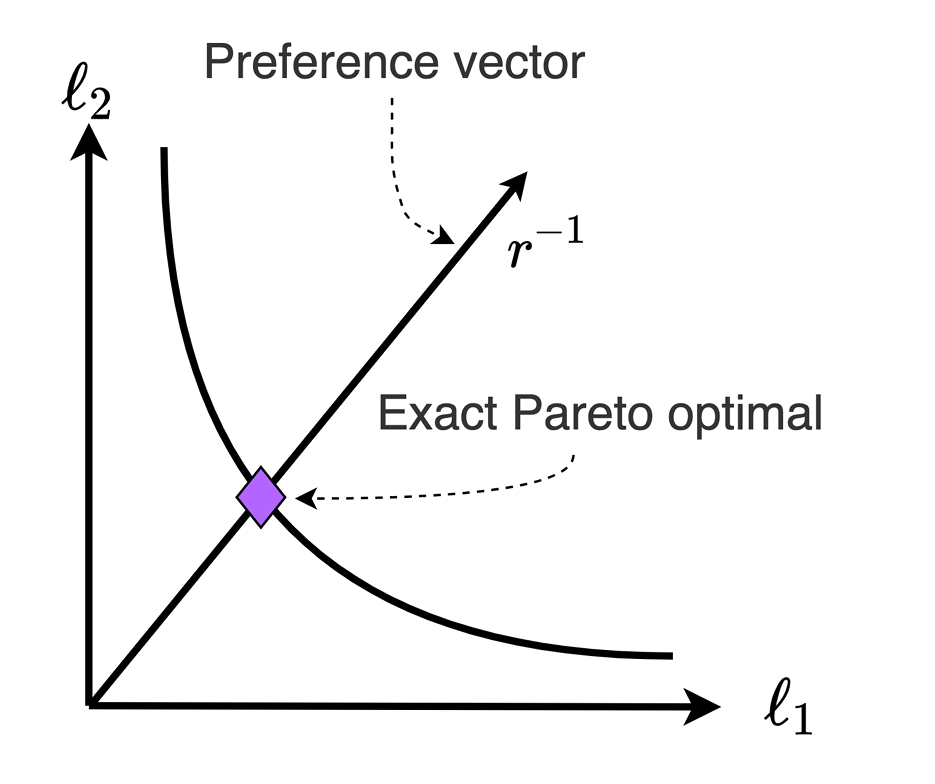
\includegraphics[width=0.5\textwidth, trim={0 0 0 0cm},clip]{images/exact_pareto.png}
\end{figure}
\end{frame}

\begin{frame}{Limitations of Previous Methods}
Previous MMO approaches have the following drawbacks
\vspace{5pt}
\begin{itemize}
\item \textbf{Scalability}: A separate model has to be trained for each point on the front. The number of models to be trained to cover the objective space grows exponentially with the number of objectives.
\item \textbf{Flexibility}: The decision maker cannot switch freely between preferences unless all models are trained and stored in advance.
%\item The exact trade-off must be known before the optimization process.
\end{itemize}
\end{frame}

\begin{frame}{Pareto Front Learning}
The goal is to design a \textbf{single} model that can be applied at inference time to \textbf{any given preference} direction, even ones not seen during training.
\vspace{5pt}
\begin{itemize}
\item Scalability: Train and store a single model
\item Flexibility: Switch trade-off points during inference
\end{itemize}
\end{frame}

\begin{frame}{Pareto HyperNetworks (PHN)}
Pareto HyperNetwork $h(\cdot; \psi)$ receives an input preference ray $\mathbf{r}$ and outputs the corresponding Pareto optimal model weights $\theta_{\mathbf{r}}$. 
\begin{figure}[h!]
    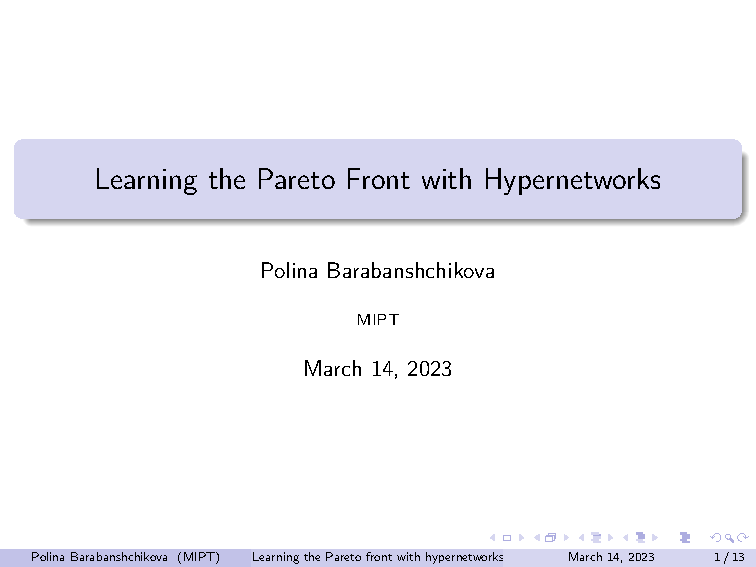
\includegraphics[width=0.8\textwidth, trim={0 0 0 0cm},clip]{images/phn.png}
\end{figure}
\end{frame}

\begin{frame}{Pseudocode} 
\begin{figure}[h!]
    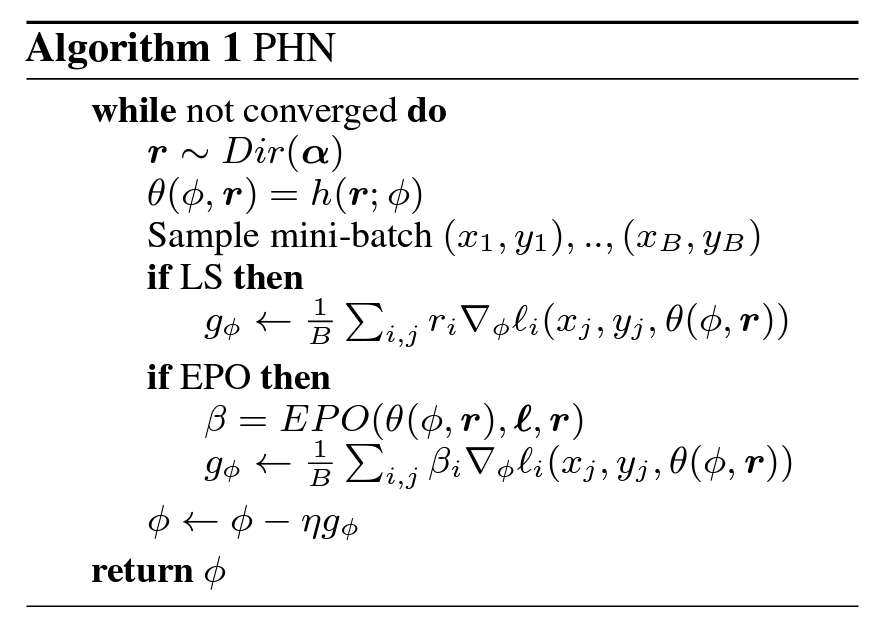
\includegraphics[width=0.5\textwidth, trim={0 0 0 0cm},clip]{images/phn_algo.png}
\end{figure}
\begin{itemize}
\item PHN-LS uses linear scalarization with the preference vector $\textbf{r}$ as loss weights, i.e the loss for input $\textbf{r}$ is $\sum_i r_i \ell_i$
\item PHN-EPO treats the preference $\textbf{r}$ as a ray in loss space and trains $\theta(\psi, \textbf{r})$ to reach a Pareto optimal point on the inverse ray $\textbf{r}^{-1}$, namely, $r_1 \cdot \ell_1 = \cdots = r_m \cdot \ell_m$.
\end{itemize}
\end{frame}

\begin{frame}{An Illustrative example}
\begin{figure}[h!]
    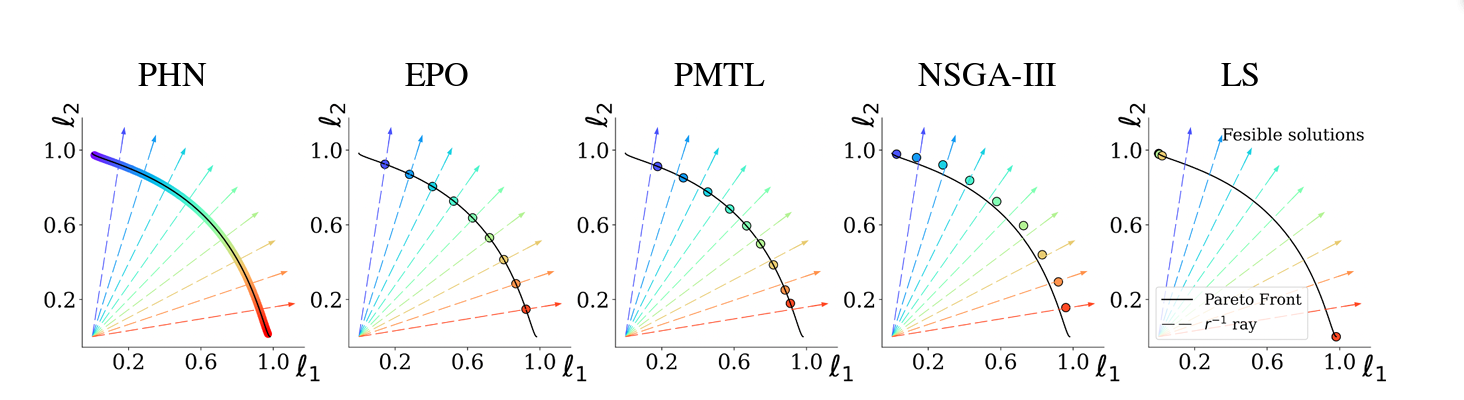
\includegraphics[width=1\textwidth, trim={0 0 0 0cm},clip]{images/pareto_example.png}
    \caption{Illustrative example using the popular task of Fonseca (1995): demonstrating the relation between Pareto front, preference rays, and solutions. Pareto front (black solid line) for a 2D loss space and several rays (colored dashed lines) which represent various possible preferences.}
\end{figure}
\end{frame}

\begin{frame}{Evaluation metrics}
\begin{itemize}
 \item \textbf{Hypervolume metric}: Given a set of points $S \subset \mathbb{R}^n$ and a reference point $\boldsymbol{\rho} \in \mathbb{R}^n_+$, the hypervolume of $S$ is measured by the region of non-dominated points bounded above by $\boldsymbol{\rho}$.
\begin{figure}[h!]
    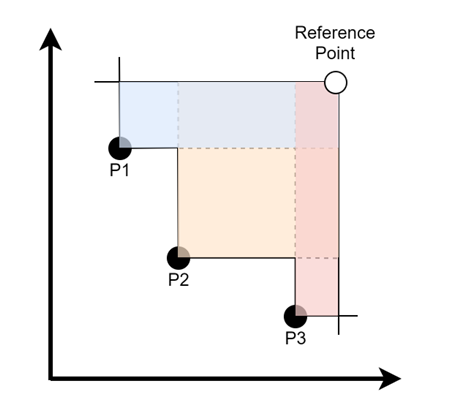
\includegraphics[width=0.3\textwidth, trim={0 0 0 0cm},clip]{images/hypervol.png}
\end{figure}
\item \textbf{Uniformity metric} quantifies how well the loss vector $\boldsymbol{\ell}(\theta)$ is aligned with the input ray $r$.
$$\mu_{\mathbf{r}}(\boldsymbol{\ell}(\theta)) = D_{KL}(\hat{\boldsymbol{\ell}} || \mathbf{1} / m), \text{ where } \hat{\boldsymbol{\ell}}_j = \frac{r_j \ell_j}{\sum_i r_i \ell_i}$$
\end{itemize}
\end{frame}

\begin{frame}{Experiments}
\textbf{Multitask classification}
\begin{figure}[h!]
    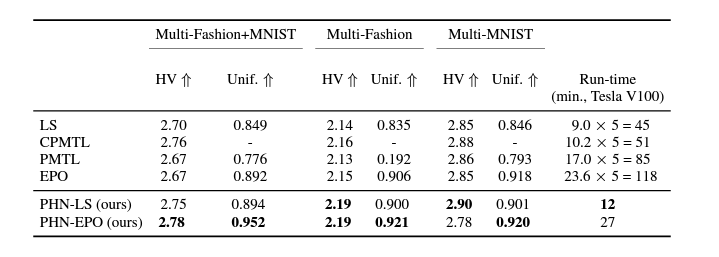
\includegraphics[width=0.6\textwidth, trim={0 0 0 0cm},clip]{images/phn_class.png}
\end{figure}
\textbf{Semantic segmentation and Depth}
\begin{figure}[h!]
    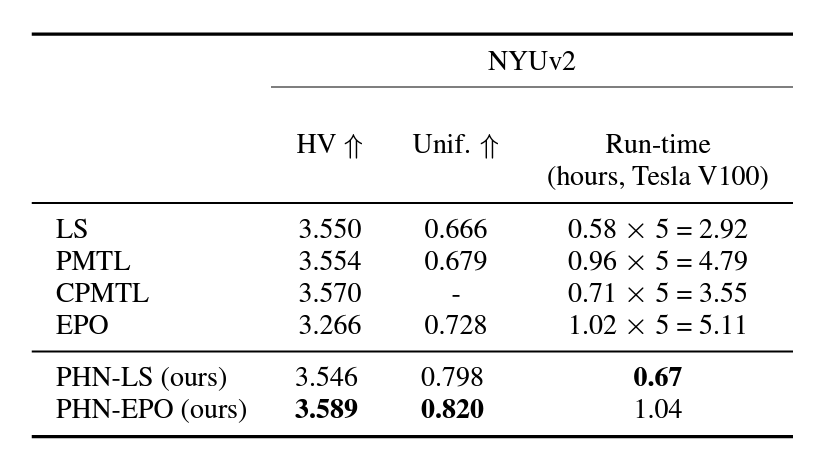
\includegraphics[width=0.4\textwidth, trim={0 0 0 0cm},clip]{images/phn_depth.png}
\end{figure}
\end{frame}

\begin{frame}{Applications}
\textbf{Fairness}

A 3-dimensional optimization problem, with a classification objective and two fairness objectives: False Positive (FP) fairness, and False Negative (FN) fairness.
\begin{figure}[h!]
    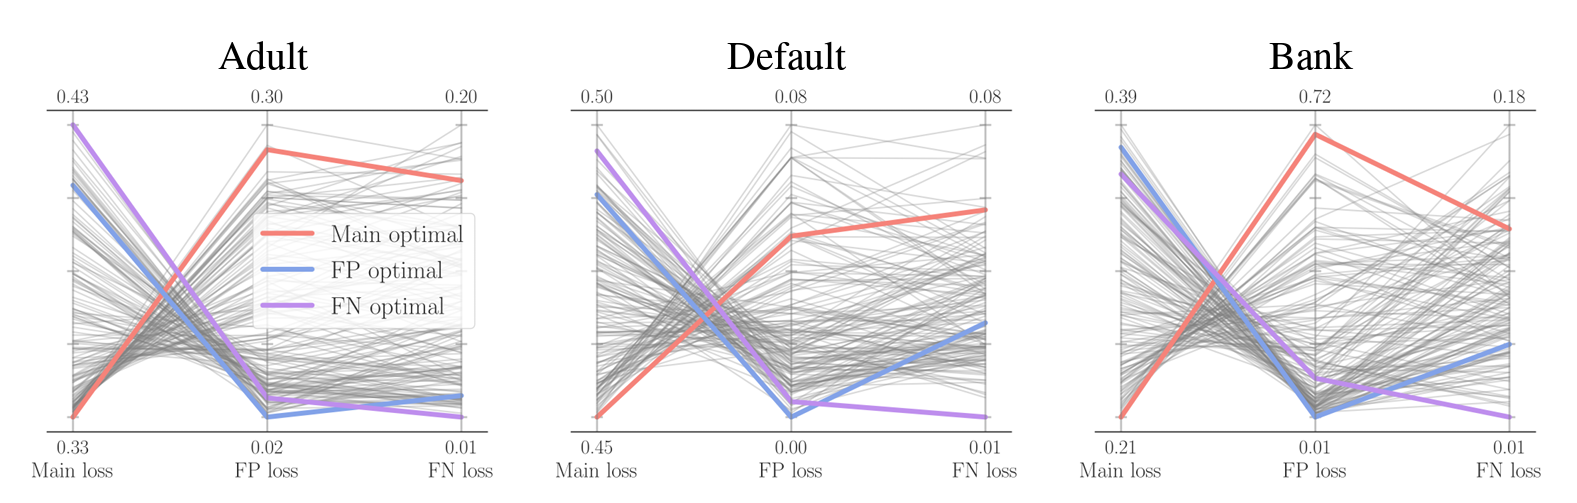
\includegraphics[width=1\textwidth, trim={0 0 0 0cm},clip]{images/fairness.png}
\end{figure}
\end{frame}

\begin{frame}{Literature}
\nocite{phn}
\printbibliography
\end{frame}


\end{document}